\section{Time plan}
% Den här delen av planeringsrapporten beskriver vad som ska göras och när det ska göras. Personer som ska kontaktas bör också stå med här. Datum eller åtminstone veckor då studenterna ska ge delrapporter samt slutgiltiga presentationen ska stå här. Tidsplanen kommer naturligtvis vara rätt grov i början.

% Det är viktigt att notera att aktiviteterna inom projektet inte kan ske helt sekventiellt eller helt parallellt då vissa aktiviteter är beroende av varandra, vilket innebär att ett antal iterationer mellan dem kommer att ske. Endast genom att iterera mellan dem kommer den uppbyggda kunskapen bli utnyttjad på ett bra sätt. Samma tänkande gäller också rapportskrivandet, det vill säga uppdatering av ett avsnitt kräver att även andra uppdateras. Rapportskrivande ska därför ske kontinuerligt under hela projektet.

For this project there are three main deadlines: the half-time presentation on the 3/5, the final deadline for the report on the 5/13, and the final presentation on the 5/24.
We also need to have made a short film about the project by the 5/15.
Figure \ref{fig:timeplan} shows our intended plan: the first weeks are mostly for research and getting started, then in the middle we will focus on developing the application and writing the report, and during the final weeks we will only focus on the report and the final presentation.
Table \ref{tab:milestones} shows the versions we have planned for the application.

\begin{table}[h]
    \centering
    \begin{tabular}{|c|p{135mm}|}
    \hline
       Version  & Description \\
       \hline
        1 & Basic web application with the ability to add qubits and single qubit gates. \\ \hline
        2 & Program can display the state vectors for each state. Also multiple qubit gates and measurement function.\\ \hline
        3 & Have well-known algorithms implemented in the program and custom gates. \\ \hline
        
    \end{tabular}
    \caption{Planned versions for the application.}
    \label{tab:milestones}
\end{table}

\begin{figure}[h]
    \centering
    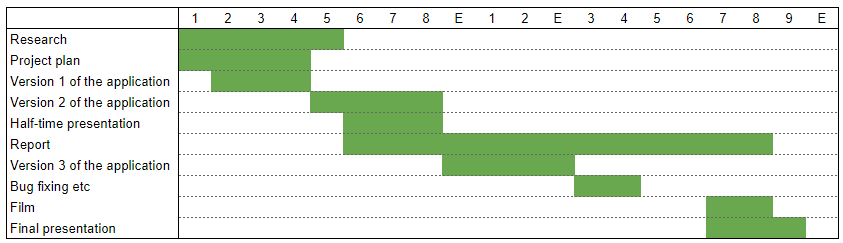
\includegraphics[scale=0.7]{assets/timePlan.PNG}
    \caption{Rough time plan for the project, the numbers are the reading weeks and "E" denote exam weeks. The application versions are explained in table \ref{tab:milestones}.}
    \label{fig:timeplan}
\end{figure}
